\section{TOCL+ Plugin Implementation}

\subsection{Plugin Architecture and Workflow}

\begin{figure}
    \centering
    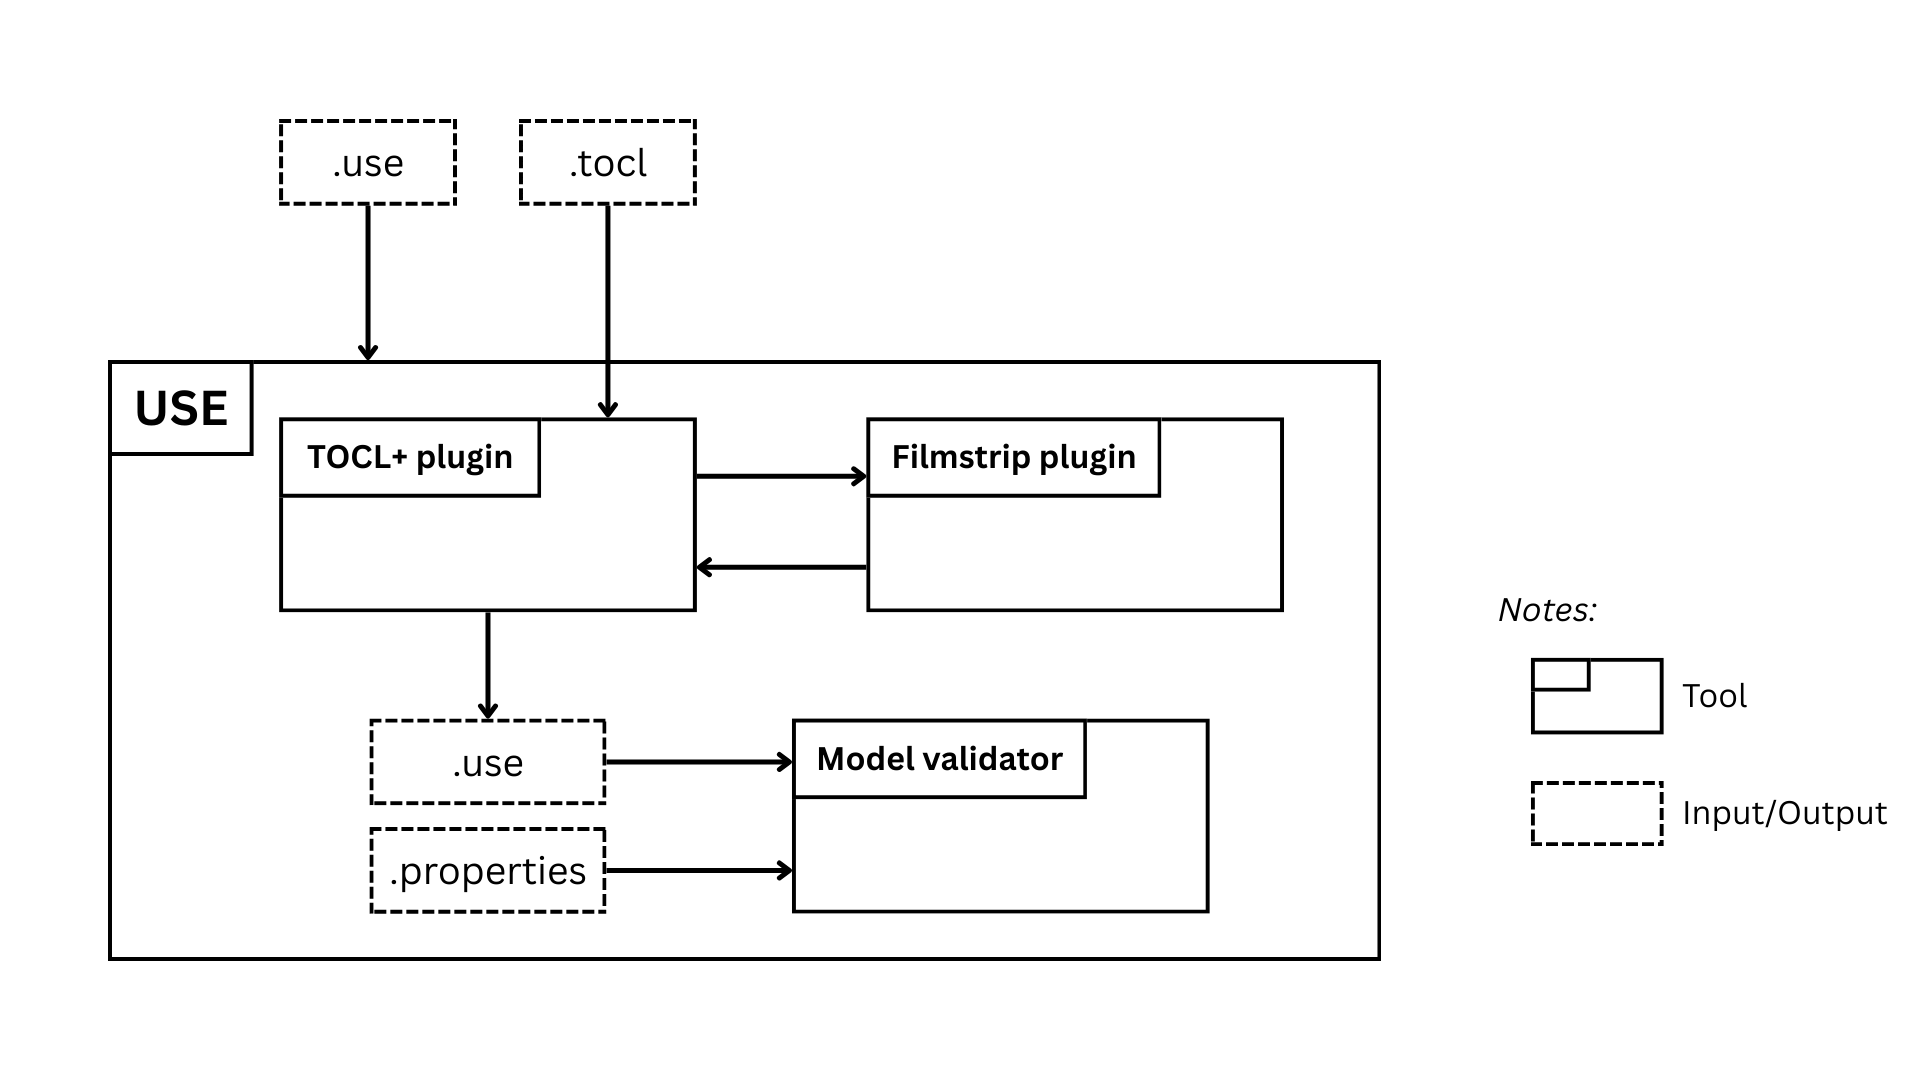
\includegraphics[width=1\textwidth]{figures/c3/Architecture_overview.png}
    \caption{Architecture and Workflow of the approach.}
    \label{sec:plugin_architecture}
\end{figure}

\hspace{1cm} Figure \ref{sec:plugin_architecture} illustrates the architecture and 
workflow of our TOCL+ plugin. The plugin integrates with the USE tool environment 
while maintaining a clear separation between modeling, specification, and 
verification concerns. The workflow consists of five distinct steps, beginning with 
preparation and ending with verification. First, the user prepares two input files: 
a standard \texttt{.use} file containing the UML/OCL application model and a 
\texttt{.tocl} file containing TOCL+ property specifications. Second, the user loads 
the application model into USE to make it available for transformation. Third, 
the user activates our plugin through the USE interface, selecting both a destination 
path for the output model and the \texttt{.tocl} file containing the temporal 
properties to verify.

Internally, the plugin then executes a two-phase transformation process. In the first 
phase, it invokes the Filmstrip plugin to transform the application model into a 
filmstrip model following the rules described in Section~\ref{subsec:filmstripping}. 
In the second phase, it processes the TOCL+ expressions using our ANTLR4-generated 
parser and listener components, which implement the transformation rules for 
converting temporal specifications into equivalent OCL constraints (detailed in the 
next subsection). These generated constraints are added to the list of invariants in 
the output model file alongside the filmstrip model elements.

To complete the verification process, the user loads this output model back into USE 
together with a configuration file that establishes search bounds, and then employs 
the Model Validator to analyze the constraints. The validator systematically explores the search space, determining whether the temporal properties are satisfied and providing a model instance as evidence when applicable. This architecture shields users from the complexities of the underlying transformation mechanisms while providing a streamlined workflow from specification to verification.


\subsection{Implementation of TOCL+ to OCL Transformation}

Using ANTLR4 listeners, we implemented the transformation as Java code built on 
the TOCL parser we created. The listeners traverse the parse tree of a TOCL+
expression and produce the corresponding OCL expression.


\begin{table}[htbp]
\caption{Translation of TOCL+ operators to OCL.}
\label{tab:TOCL2OCL}
\begin{tabularx}{\textwidth}{|>{\footnotesize}p{0.8cm}|>{\scriptsize\raggedright\arraybackslash}p{4cm}|>{\scriptsize\raggedright\arraybackslash}X|}
    \hline
    \textbf{No.} & \textbf{TOCL+} & \textbf{OCL Translation} \\
    \hline
    1 & 
    next P &
    let nextSnapshot:Snapshot = self.snapshot.succ() in [nextSnapshot |= P] \\
    \hline
    2 &
    always P &
    let CS:Snapshot = self.snapshot in Set\{CS\}->closure(s | s.succ())->forAll(s | [s |= P]) \\
    \hline  
    3 &
    always P until Q &
    let CS:Snapshot = self.snapshot
    in let FS:Set(Snapshot) = Set\{CS.succ()\}->closure(s | s.succ())
    in let AllFSQ:Set(Snapshot) = FS->select(s | [s |= Q])
    in let FSQ:Snapshot = AllFSQ->any(s | Set\{s\}->closure(s | s.succ())->includesAll(AllFSQ))
    in let afterQ:Set(Snapshot) = Set\{FSQ\}->closure(s | s.succ())
    in let FSP:Set(Snapshot) = FS->select(s | [s |= P])
    in if FSQ.isDefined() then (if (FSP->size() > 0) then (FS-afterQ = FSP-afterQ) else false endif) else (FS = FSP) endif \\
    \hline
    4 &
    always P since Q &
    let CS:Snapshot = self.snapshot
    in let PS:Set(Snapshot) = Set\{CS.pred()\}->closure(s | s.pred())
    in let AllPSQ:Set(Snapshot) = PS->select(s | [s |= Q])
    in let PSQ:Snapshot = AllPSQ->any(s | Set\{s\}->closure(s | s.pred())->includesAll(AllPSQ))
    in let beforeQ:Set(Snapshot) = Set\{PSQ\}->closure(s | s.pred())
    in let PSP:Set(Snapshot) = PS->including(CS)->select(s | [s |= P])
    in if PSQ.isDefined() then (if (PSP->size() > 0) then (PS->including(CS)-beforeQ = PSP-beforeQ) else false endif) else (PSP = PS->including(CS)) endif \\
    \hline
    5 &
    sometime P &
    let CS:Snapshot = self.snapshot in Set\{CS\}->closure(s | s.succ())->exists(s | [s |= P]) \\
    \hline
    6 &
    sometime P before Q &
    let FS:Set(Snapshot) = Set\{self.snapshot\}->closure(s | s.succ())
    in let PreS:Set(Snapshot) = Set\{self.snapshot.pred()\}->closure(s | s.pred())
    in let AllFSQ:Set(Snapshot) = FS->select(s | [s |= Q])
    in let FSQ:Snapshot = AllFSQ->any(s | Set\{s\}->closure(s | s.succ())->includesAll(AllFSQ))
    in let FSP:Set(Snapshot) = FS->select(s | [s |= P])
    in if FSQ.isDefined() then (if (FSP->size() > 0) then ((Set\{FSQ.pred()\}->closure(s | s.pred())-PreS)->exists(s\_1 | FSP->includes(s\_1))) else false endif) else false endif \\
    \hline
    7 &
    sometime P since Q &
    let CS:Snapshot = self.snapshot
    in let PS:Set(Snapshot) = Set\{CS.pred()\}->closure(s | s.pred())
    in let AllPSQ:Set(Snapshot) = PS->select(s | [s |= Q])
    in let PSQ:Snapshot = AllPSQ->any(s | Set\{s\}->closure(s | s.pred())->includesAll(AllPSQ))
    in let PSP:Set(Snapshot) = PS->select(s | [s |= P])
    in if PSQ.isDefined() then (Set{PSQ}->closure(s | s.succ())->excluding(null)->intersection(PS)->exists(s | PSP->includes(s))) else false endif \\ 
    \hline
    8 &
    previous P &
    let previousSnapshot:Snapshot = self.snapshot.pred() in [previousSnapshot |= P] \\
    \hline
    9 &
    sometimePast P &
    let CS:Snapshot = self.snapshot in Set\{CS.pred()\}->closure(s | s.pred())->exists(s | [s |= P]) \\
    \hline
    10 &
    alwaysPast P &
    let CS:Snapshot = self.snapshot in Set\{CS.pred()\}->closure(s | s.pred())->forAll(s | [s |= P]) \\
    \hline
\end{tabularx}
\end{table}
